\section{Balance Workload}
Whenever a staff is removed from a department or has finished solving a problem. 
It is necessary to balance the workload of each staff in the department, since we do not want the staffs to be overloaded with problems. 

To balance the workload, each staffs workload must be calculated. 
The workload of a staff is defined by the amount of time estimated that each problem on his workload takes to be solved. 
The workload is calculated by the \me{GetWorkload} method.

The time a problem takes to be solved is estimated by the average time consumption of the tags connected to the problem. 
This is calculated by the \me{CalculateTimeConsumption} method.

The \me{BalanceWorkload} method works by finding the staff in the department with the minimum workload and the staff with the maximum workload. T
hen it moves the highest priority problems from the maximum staff to the minimum. 
It keeps reassigning problems until the minimum staff has a higher or equal workload than the maximum staff. If it is higher the problem is reassigned back. 
All this is iterated once per staff minus one in the department. 
E.g. if there are two staffs it is run once, if there is three it yields two etc. 
The pseudo code is display in code snippet \ref{lst:balanceWorkload}.

The primary concern of the algorithm is to distribute the problems so each staff has as balance a workload as possible. 
This balance is based on the time approximated that all problems on his workload consumes. 
We also wanted the algorithm to take the individual priority of the problems into account. 
This algorithm makes sure that the high priority problems will be distributed. 
If the priority was unrelevant the algorithm would take the problem with lowest time consume, since this would give the most balanced workload. 
An example of the algorithm is shown on figure \ref{fig:balanceWorkloadDiagram}. 

%There is one weakness though and that is if a staff has a highly time consuming problem with low priority. Then he will be left with only that problem. Assuming it is as time consuming as all the other problems. 


\begin{figure}
	\centering
		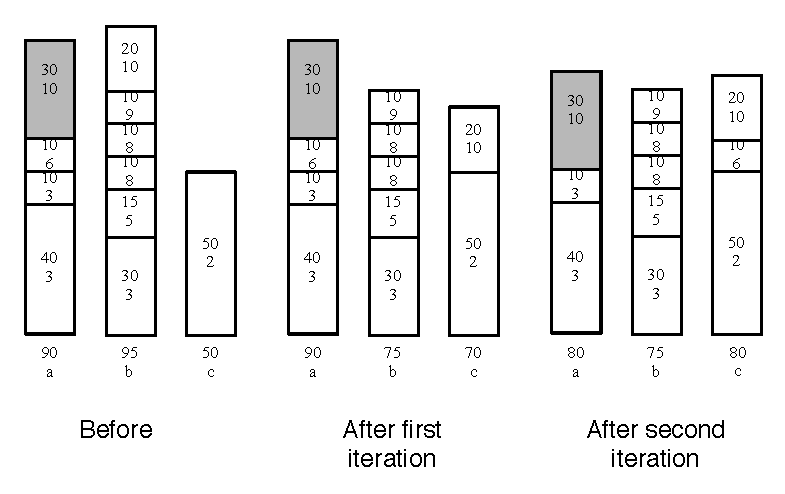
\includegraphics[scale=0.8]{input/implementation/key_points/balanceWorkloadDiagram.pdf}
	\morscaption{A diagram of the balance workload method. Each collum represents a staffs workload. Each box is a problem. The upper number is the estimated time consumed of that problem. The lower is the priority. The problem colored dark grey is not reassignable.  There are tree staffs a, b, and c. The problems that will be moved is colored light grey. }
	\label{fig:balanceWorkloadDiagram}
\end{figure}


\begin{lstlisting}[style=sourceCode, caption=\myCaption{To be}, label=lst:balanceWorkload]
var max = Persons.FirstOrDefault(y => 	
		y.GetWorkload() == Persons.Max(x => 
		x.GetWorkload()));                  

var min = Persons.FirstOrDefault(y => 
		y.GetWorkload() == Persons.Min(x => 
		x.GetWorkload()));
    
max.Worklist.ToList().Sort(Problem.GetComparer());             
while(true)
{
    var problemToBeMoved = max.Worklist.FirstOrDefault(y => 
		y.Reassignable == true && 
		y.HasBeen == false && 
		y.SolvedAtTime == null);
                   
    if (problemToBeMoved == null)     break; 
    problemToBeMoved.HasBeen = true;
    problemToBeMoved.AssignedTo = min;
    
    if (min.Workload > max.Workload)
    {
    	problemToBeMoved.AssignedTo = max;
    	break;
    }
    else if (min.Workload == max.Workload)
    {
		break;
    }
} 
\end{lstlisting}




\subsection{eta}
\label{}


Get workload kalder ETA